%!TEX root = ../../super_main.tex

%lad være med at sætte 2 l'er ind. Det her er US spelling
\section{Modeling Sensor Data}
\label{sec:modeling_sensor_data}

Conceptually, a \emph{snapshot} is a snippet of the reality (context) that a specific participants exists in, measured through the subjects devices, along with a \emph{label}, describing this reality further. This label is used to define the reality in ways that available sensors cannot. By examining the measured reality and the labels describing these measurements, customers will be able to recognize patterns, and be able to see a correlation between sensor output and human dynamics. To see development of patterns in time, multiple measurements might be required, e.g. measuring changes in acceleration to see that a user is speeding up. To facilitate this, a snapshot consists of a sequence of sensor readings collected from multiple sensors and a label. In order to see this development over time, time has to pass between every measurement. This timespan depends on what the customer desired to measure, and therefore he/she must be able to configure how long we wait between every sensor reading. In order to define this timespan, and other things such as which sensors to measure from, and when to present the questionnaire to the participants, the customers must define what we call a \emph{campaign}.
\\\\
One could imagine that a customer might be interested in finding a correlation between heart rate and movement patterns and the influence of alcohol. To do this, a customer could specify a campaign, which should collect information regarding sensors such as \emph{heart rate}, \emph{accelerometer}, and \emph{GPS location}. To know if the participants have consumed alcohol, the customer would specify that participants should indicate if they are, or have been, under the influence of alcohol at a specific time. When contributing information to this campaign, participants would submit snapshots matching this specification. An illustration of how these snapshots are structured can be seen in \figref{fig:snapshot_model_no_samples}, where it can be seen how time elapses between every measurement, which has been configured by the customer. In this example, the participants are asked to label the snapshot by answering the question \emph{Are you under the influence by alcohol?}.
\\
\begin{figure}[!htbp]
    \centering
    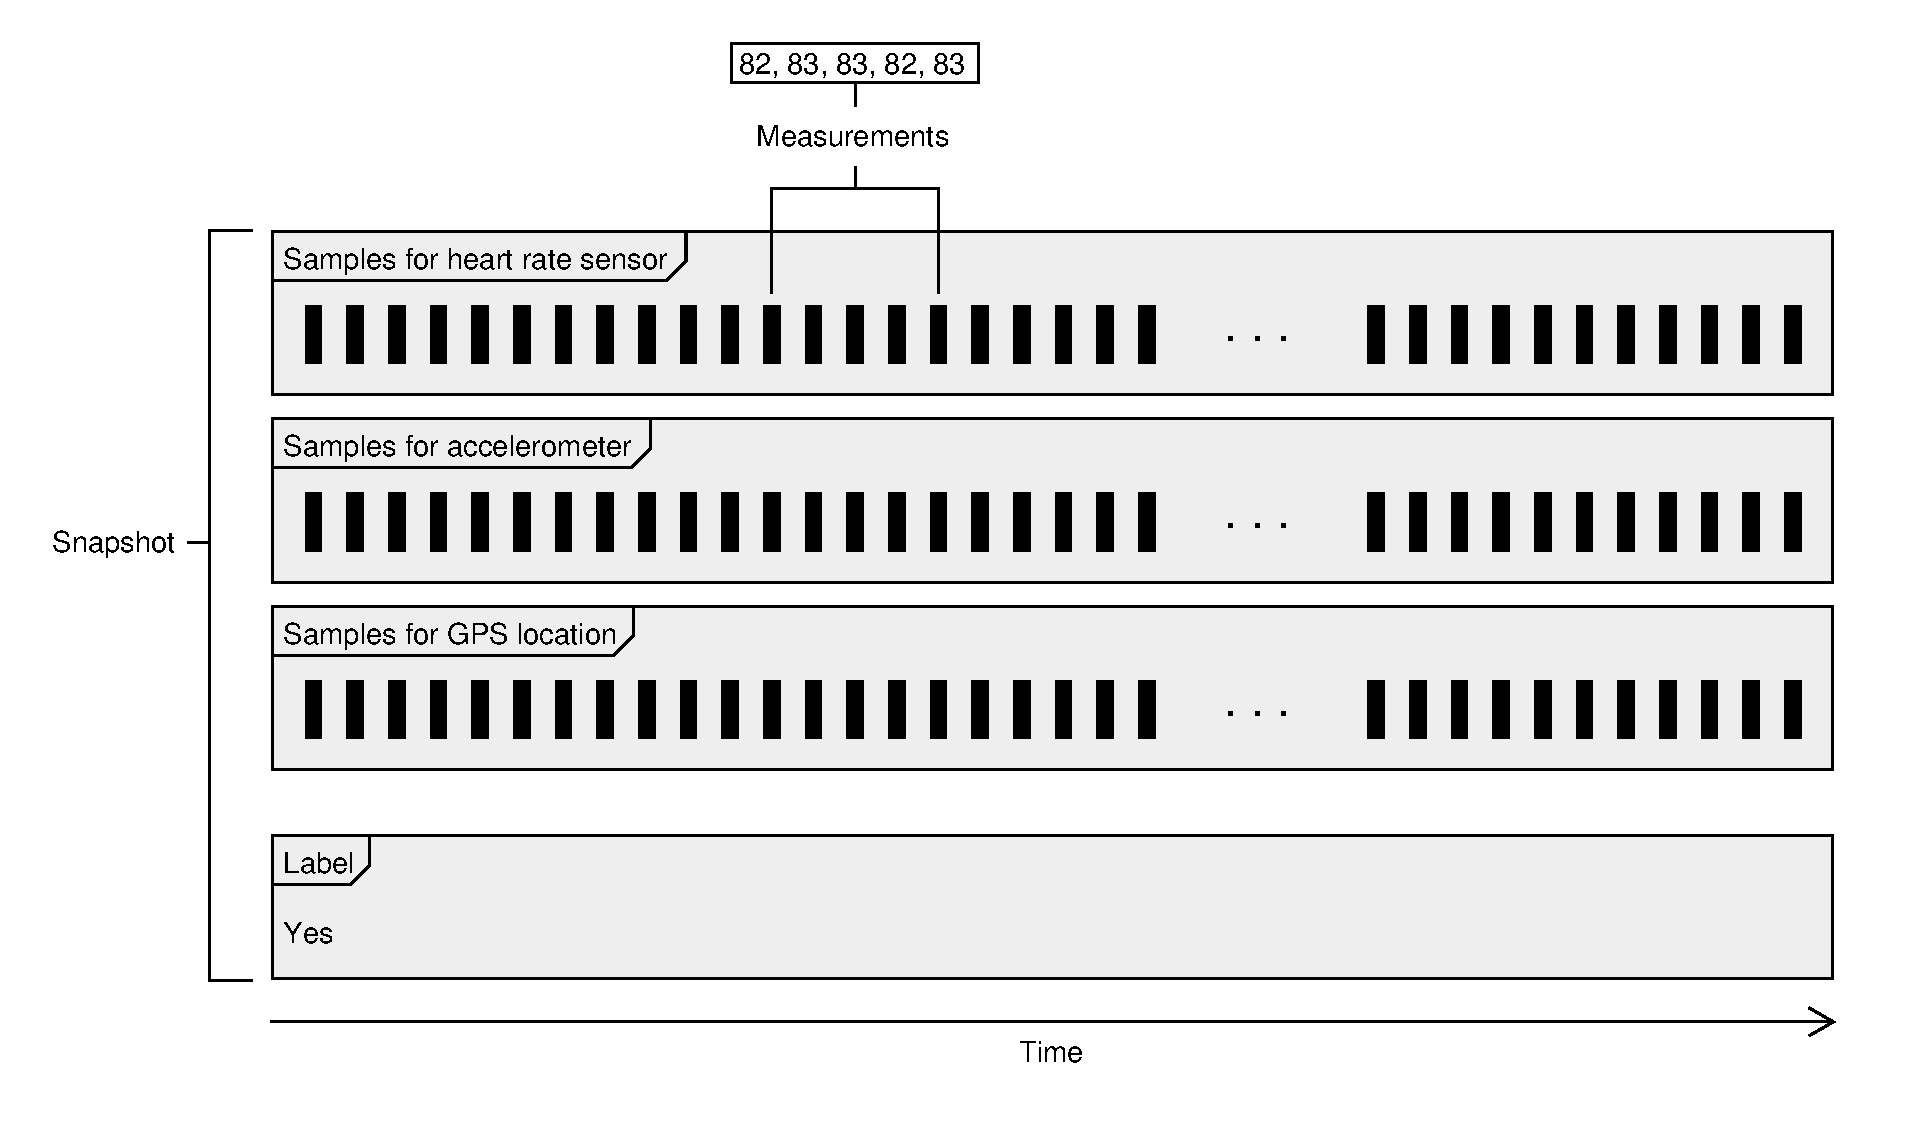
\includegraphics[width=\textwidth]{gathering_sensor_data/snapshot_model_no_samples}
    \caption{Snapshot example containing measurements from three sensors and a label.}
    \label{fig:snapshot_model_no_samples}
\end{figure}
\FloatBarrier

\subsection{Temporal Properties of Snapshots}
\label{sec:temporal_properties_of_snapshots}

A single sensor reading from a continuous sensor often does not make much sense on its own, which is why we introduced the \emph{measurement} concept. Following the introduction of measurements, we came to the realization that customers might be interested in taking a stream of measurements, waiting for some amount of time, and then taking a new stream of measurements. This has led to the introduction of a concept that we call \emph{sample}. A \emph{sample} is simply a collection of \emph{measurement}s where there is an interval between them, as seen in \figref{fig:snapshot_example_with_samples}. This allows customers to make sense of continuous sensor readings, but in a periodic manner. 

\begin{figure}[!htbp]
    \centering
    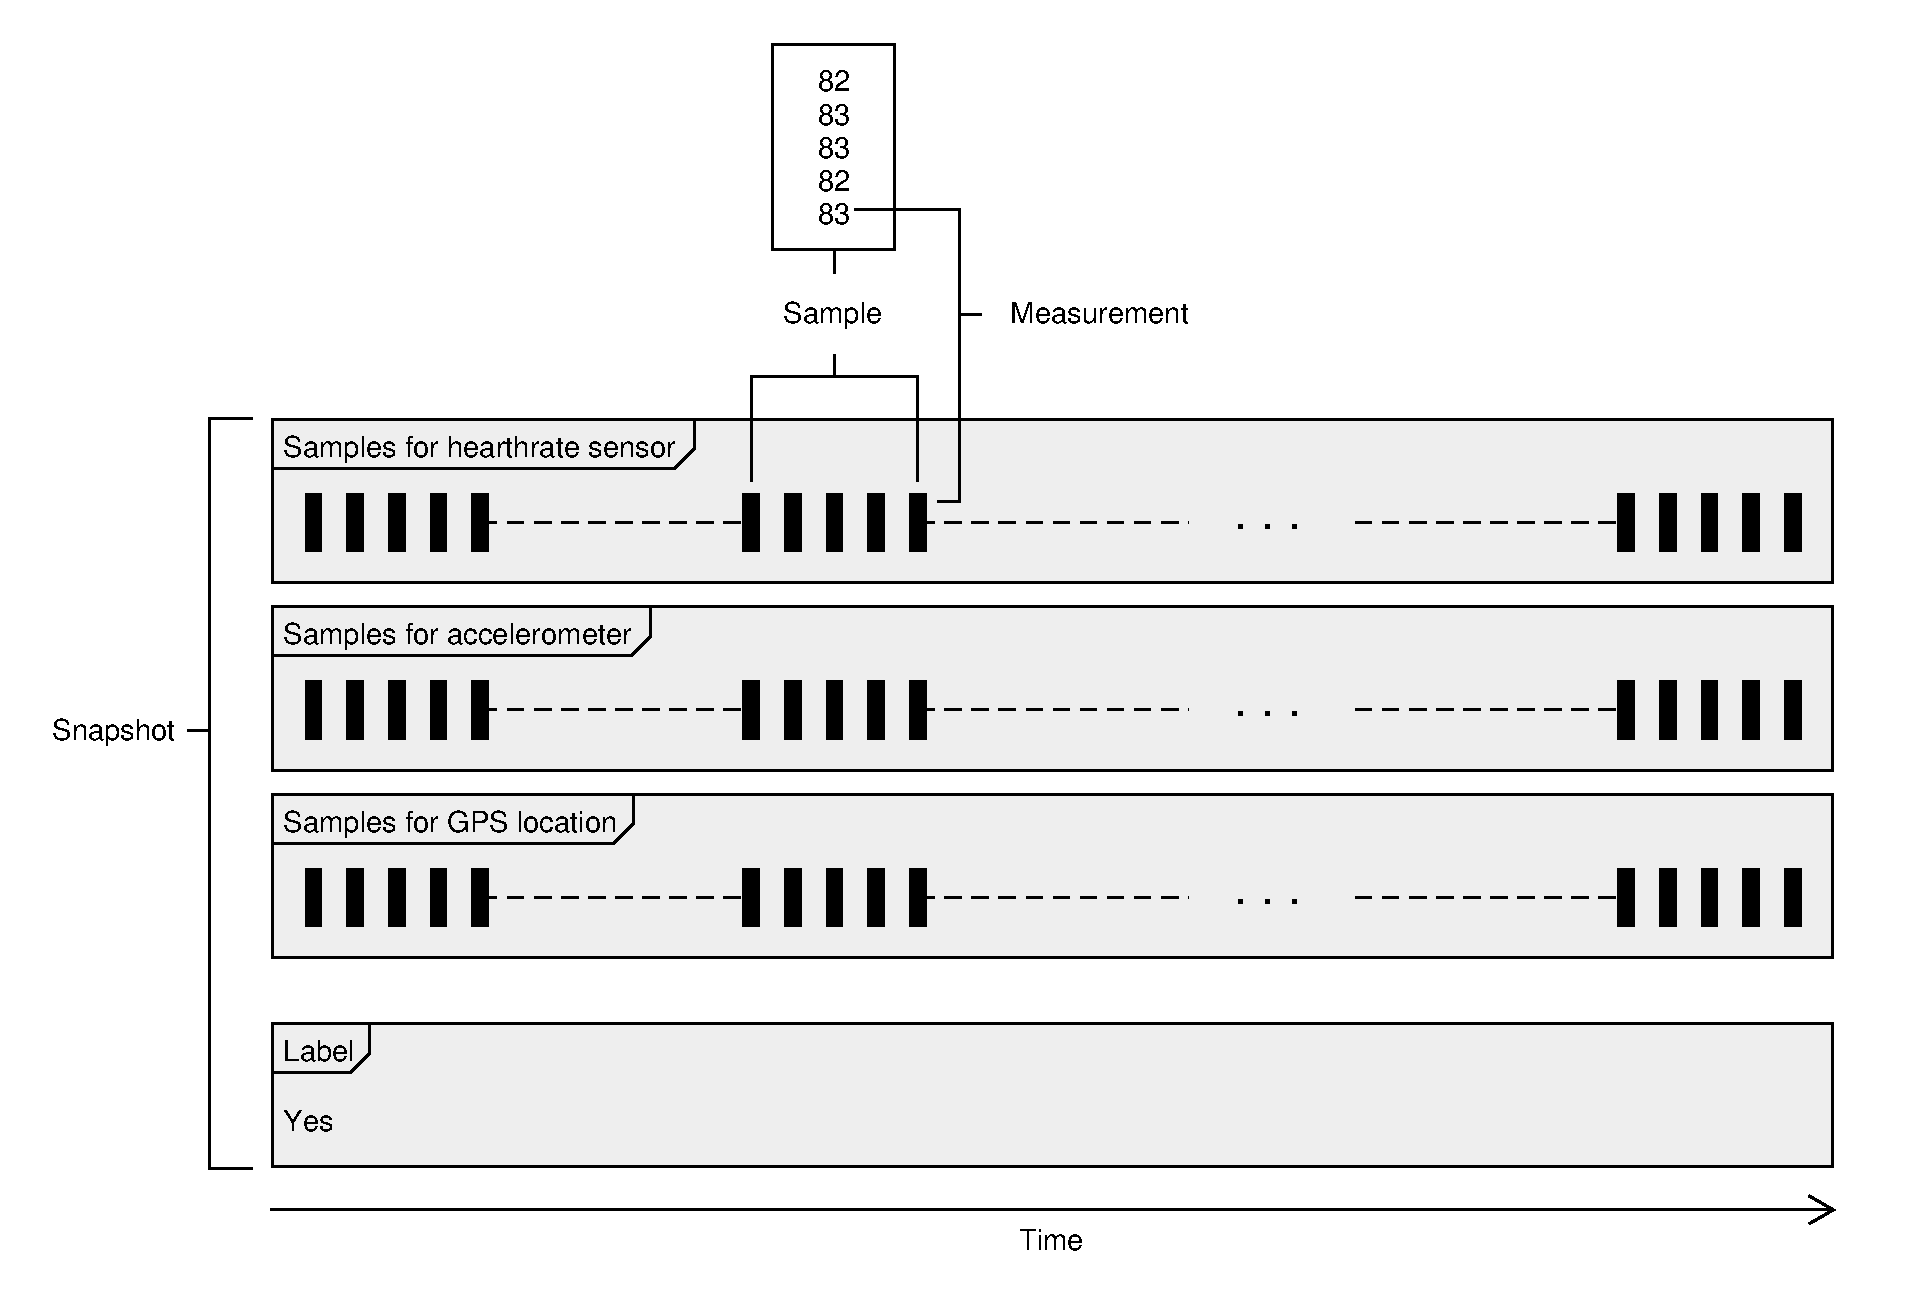
\includegraphics[width=\textwidth]{gathering_sensor_data/snapshot}
    \caption{Snapshot example containing samples from three sensors and a label.}
    \label{fig:snapshot_example_with_samples}
\end{figure}
\FloatBarrier

We want customers to configure how often \emph{measurement}s should be made, and we therefore allow them to define a \emph{measurement frequency} for their \emph{campaign}. Customers should furthermore be able to define how often \emph{sample}s should be gathered, and for that reason we allow them to define a \emph{sample frequency}. And lastly the length of the \emph{snapshot} is configurable by defining how many \emph{sample}s the customer wants for a single \emph{snapshot}, which then behind the scenes is used to calculate what we call \emph{total duration}, which states for how long samples should be generated for a snapshot. All of this is illustrated in \figref{fig:sample_temporality}. 

\begin{figure}[!htbp]
    \centering
    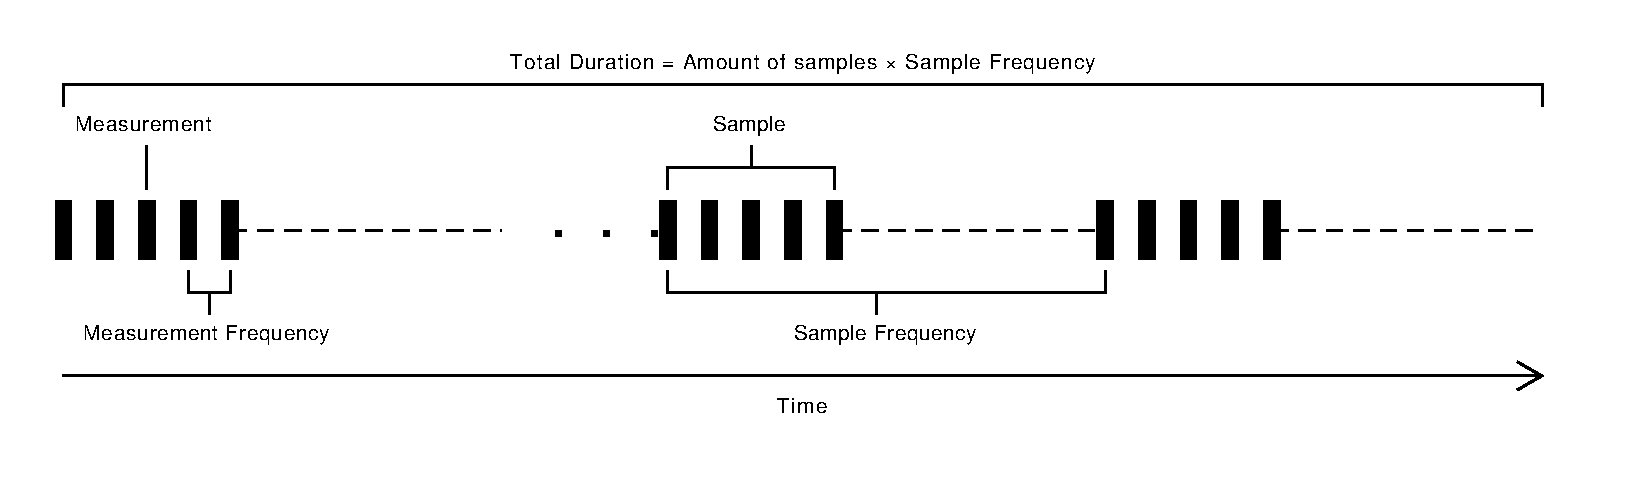
\includegraphics[width=\textwidth]{gathering_sensor_data/sample_temporality}
    \caption{Illustration of temporality for samples for a single sensor in a snapshot.}
    \label{fig:sample_temporality}
\end{figure}
\FloatBarrier

By this temporal structure of the sensor data we provide a viable way of configuring how the snapshots should be structured in regards to sensor readings, while maintaining a uniform output format for customers of the system.
